\subsection{Modeling}
\label{sec:modeling}
Throughout the past few decades, numerous modeling languages and tools have been introduced, for example ...\danielle{examples and citations}. As described in Section 2.1.3, the digital and mechanical components of a system can be described in abstract form; furthermore, the requirements of the system and of each component can be specified in formal logic. The verification of such models take both the architecture and the requirement specification into account when analyzing the behavior and interactions of the components comprising the system. The following sections describe aspects of modeling that are pertinant to this research.

\subsubsection{State Machines}
A state machine (or state automaton) is a mathematical model of computation and consists of states, represented by nodes, and transitions between them, represented by directed edges. The change from one state to another is called a {\em transition}. State machines may be finite (can only be in a finite number of states at a time) or infinite. %The expressive capabilities of set notation and predicate logic allow finite strings to represent infinite states, which are much more expressive. For example, the infinite set of integers greater than zero is described succinctly as: $\{x \in \mathbb{Z} : x > 0\}$. 
Model checkers often utilize the expressive power of state machines to verify specifications. One such example important to this thesis is JKind~\cite{2017arXiv171201222G}, an infinite state model checker. Verification of the program is based on {\em k-induction} (see Section~\ref{sec:induction}) and property directed reachability using a back-end SMT solver such as Z3~\cite{z3} or SMTInterpol~\cite{smtInterpol}. 

To reason about state machines, transitions between the states must be defined and analyzed.

\subsubsection{Transition Systems and Reachability}
Transition systems are directed graphs with nodes representing reachable states and edges representing transitions between them. In this research we consider \emph{safety properties} over infinite-state machines. The states are vectors of variables that define the values of state variables. We assume there are a set of legal \emph{initial states} and the safety property is specified as a formula over state variables. A \emph{reachable state space} means that all states are reachable from the initial state. 

Given a state space $U$, a transition system $(I,T)$ consists of an
initial state predicate $I : U \to \bool$ and a transition step
predicate $T : U \times U \to \bool$.
We define the notion of
reachability for $(I, T)$ as the smallest predicate $\reach : U \to
\bool$ which satisfies the following formulas:
\begin{gather*}
  \forall u.~ I(u) \Rightarrow \reach(u) \\
  \forall u, u'.~ \reach(u) \land T(u, u') \Rightarrow \reach(u')
\end{gather*}
A safety property $P : U \to \bool$ is a state predicate. A safety
property $P$ holds on a transition system $(I, T)$ if it holds on all
reachable states, i.e., $\forall u.~ \reach(u) \Rightarrow P(u)$,
written as $\reach \Rightarrow P$ for short. When this is the case, we
write $(I, T)\vdash P$.

\subsubsection{Induction}
\label{sec:induction}
For an arbitrary transition system $(I, T)$, computing reachability
can be very expensive or even impossible. Thus, we need a more
effective way of checking if a safety property $P$ is satisfied by the
system. The key idea is to over-approximate reachability. If we can
find an over-approximation that implies the property, then the
property must hold. Otherwise, the approximation needs to be refined.

A good first approximation for reachability is the property itself.
That is, we can check if the following formulas hold:
\begin{gather}
  \forall s.~ I(s) \Rightarrow P(s)
  \label{eq:1-ind-base} \\
  \forall s, s'.~ P(s) \land T(s, s') \Rightarrow P(s')
  \label{eq:1-ind-step}
\end{gather}
If both formulas hold then $P$ is {\em inductive} and holds over the
system. If (\ref{eq:1-ind-base}) fails to hold, then $P$ is violated
by an initial state of the system. If (\ref{eq:1-ind-step}) fails to
hold, then $P$ is too much of an over-approximation and needs to be
refined.

The JKind model checker~\cite{2017arXiv171201222G} used in this research uses {\em
  $k$-induction} which unrolls the property over $k$ steps of the
transition system. For example, 1-induction consists of formulas
(\ref{eq:1-ind-base}) and (\ref{eq:1-ind-step}) above, whereas
2-induction consists of the following formulas:
\begin{gather*}
\forall s.~ I(s) \Rightarrow P(s) \\
\forall s, s'.~ I(s) \land T(s, s') \Rightarrow P(s') \\
\forall s, s', s''.~ P(s) \land T(s, s') \land P(s') \land T(s',
  s'') \Rightarrow P(s'')
\end{gather*}
That is, there are two base step checks and one inductive step check.
In general, for an arbitrary $k$, $k$-induction consists of $k$
base step checks and one inductive step check as shown in
Figure~\ref{fig:k-induction} (the universal quantifiers on $s_i$ have
been elided for space). We say that a property is $k$-inductive if it
satisfies the $k$-induction constraints for the given value of $k$.
The hope is that the additional formulas in the antecedent of the
inductive step make it provable.

\begin{figure}
\begin{gather*}
I(s_0) \Rightarrow P(s_0) \\[-2pt]
%
\vdots \\[2pt]
%
I(s_0) \land T(s_0, s_1) \land \cdots \land T(s_{k-2}, s_{k-1})
\Rightarrow P(s_{k-1}) \\[2pt]
%
P(s_0) \land T(s_0, s_1) \land \cdots \land P(s_{k-1}) \land
T(s_{k-1}, s_k) \Rightarrow P(s_k)
\end{gather*}
\caption{$k$-induction formulas: $k$ base cases and one inductive
  step}
\label{fig:k-induction}
\end{figure}

In practice, inductive model checkers often use a combination of the
above techniques. Thus, a typical conclusion is of the form ``$P$ with
lemmas $L_1, \ldots, L_n$ is $k$-inductive''.


\begin{comment}
\subsubsection{Ordered Binary Decision Diagrams}
A Binary Decision Diagram (BDD) is a data structure used to encode Boolean formulae.
\begin{figure}[htbp]
        \center{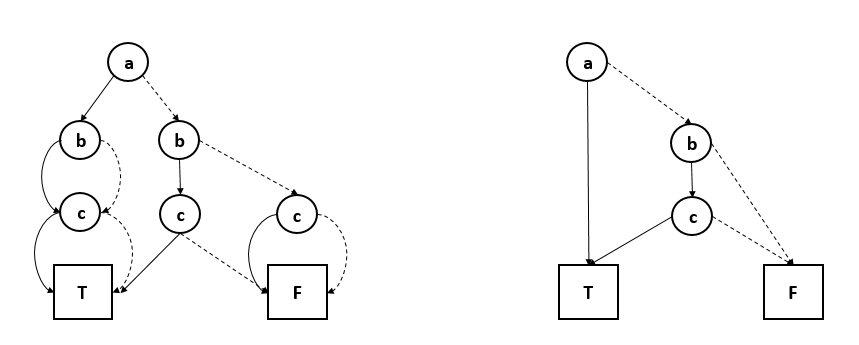
\includegraphics[width=0.8\textwidth] {images/bdd.png}}
        \caption{\label{fig:bdd} Binary Decision Diagrams of the Formula $a \lor (b \land c)$}
\end{figure}
As shown in Figure~\ref{fig:bdd}, it is a rooted, directed, acyclic graph with internal decision nodes and two terminal nodes (\textit{true} and \textit{false}). Each of the decision nodes is labeled with a Boolean variable and has two child nodes, low child and high child. The edge from a node to its low child represents the assignment of \textit{false}, likewise the edge to the high child represents the assignment of \textit{true}. The BDD is called \textit{ordered} if different variables appear in the same order on all paths from the root. Intuitively, following a path from the root to the \textit{true} terminal node represents a valid assignment to the Boolean formula (invalid in the case of ending on the \textit{false} terminal node). 

BDDs are reduced by the removal of isomorphic subgraphs. The BDD shown on the right of Figure~\ref{fig:bdd} is the reduced form of the BDD on the left.
\end{comment}